\graphicspath{{2groups/asy/},{3cyclic/asy/},{1intro/asy/}}

\section{Group Axioms and Basic Examples}\label{chap:groups}

In this chapter we define our main objects of study and introduce some of the vocabulary and standard examples used throughout the course. The ``Key concepts/definitions'' listed at the start of each Exercise set summarize these.


\subsection{The Axioms of a Group}\label{sec:groupaxioms}

\begin{defn}{Closure}{}
	Let $G$ be a set and $*$ a function $*:G\times G\to G$. We describe this arrangement in four different ways, though all mean exactly the same thing:
	\begin{enumeratea}\itemsep2pt
	  \item \makebox[230pt][l]{$\forall x,y\in G, \ x\opast y\in G$ \hfill (b) }
	  $G$ is \emph{closed} under $*$.
	  \setcounter{enumi}{2}
	  \item \makebox[230pt][l]{$*$ is a \emph{binary operation} on $G$. \hfill (d) }
	  $(G,*)$ is a \emph{binary structure.}
	\end{enumeratea}
\end{defn}


In abstract situations (including most theorems) we typically drop the $\ast$ symbol and use \emph{juxtaposition} ($x\opast y=xy$). In explicit \emph{examples} this might be a bad idea, say if $*$ is addition\ldots

\begin{examples}{}{basicexs}
	\exstart Addition ($+$) is a binary operation on the set of \emph{integers} $\Z$:\vspace{-2pt}
	\begin{enumerate}\setcounter{enumi}{1}
		\item[]\begin{quote}
			Given $x,y\in\Z$, we know that $x+y\in\Z$
		\end{quote}
		\smallskip
		This isn't a claim you can \emph{prove}, since it is really part of the \emph{definition} of integer addition.

	  \item Subtraction ($-$) is \emph{not} a binary operation on the positive integers $\N=\{1,2,3,4,\ldots\}$. This you can prove; to show that condition (a) is \emph{false,} we exhibit a \emph{counter-example}
	  \[
	  	1-7=-6\not\in\N\tag{$\exists x,y\in\N$ such that $x-y\not\in\N$}
	  \]
	  On the integers, however, subtraction is a binary operation: $\Z$ is closed under $-$.
  
	 	\begin{minipage}[t]{0.8\linewidth}\vspace{0pt}
		  \item\label{ex:table1} On a small set, it can be convenient to represent a binary operation in tabular form. The given table describes an operation $*$ on a set of three elements $G=\{e,a,b\}$. Read the  \emph{left} column first, then the \emph{top} row: for instance,
		  \[
		  	\textcolor{red}{a}*\textcolor{blue}{b}=\textcolor{Green}{e},
		  	\ \text{ or simply }\
		  	\textcolor{red}{a}\textcolor{blue}{b}=\textcolor{Green}{e}
		  \]
		\end{minipage}
		\hfill
		\begin{minipage}[t]{0.15\linewidth}\vspace{0pt}
			\flushright
			$\begin{array}{c||c|c|c}
				* & e & a & \textcolor{blue}{b}\\\hline\hline
				e & e & a & b\\\hline
				\textcolor{red}{a} & a & e & \textcolor{Green}{e}\\\hline
				b & b & e & a
			\end{array}$
		\end{minipage}
	\end{enumerate}
\end{examples}


We'll continue checking these examples for each of the remaining axioms.


\begin{defn}{Associativity}{assoc}
	A binary structure $(G,\ast)$ is \emph{associative} if
	\[
		\forall x,y,z\in G,\ x(yz)=(xy)z
	\]
	If $\ast$ is associative, then the expression $x y z$ has unambiguous meaning, as does  \emph{exponential} notation:\ $x^n=x\cdots x$ ($n$ factors).
\end{defn}

\begin{examples*}{\ref{ex:basicexs}, ver.\,II}{}
	\exstart Addition is associative: $x+(y+z)=(x+y)+z$ for any integers.\vspace{-2pt}
	\begin{enumerate}\setcounter{enumi}{1}%\itemsep2pt
	  \item $(\Z,-)$ is non-associative: e.g.\ $(1-3)-2=-4$, but $1-(3-2)=0$.
	  \item $\bigl(\{e,a,b\},*\bigr)$, described in the table, is non-associative: e.g.\ $a(bb)=aa=e$, but $(ab)b=eb=b$.
	\end{enumerate}
\end{examples*}

\goodbreak

\begin{defn}{Identity}{}
	A binary structure $(G,\ast)$ has an \emph{identity element} $e\in G$ if
	\[
		\forall x\in G,\ ex=xe=x
	\]
\end{defn}

\begin{examples*}{\ref{ex:basicexs}, ver.\,III}{}
	\exstart Addition on $\Z$ has identity 0, since $0+x=x+0=x$ for any integer $x$.
	\begin{enumerate}\setcounter{enumi}{1}%\itemsep2pt
	  \item $(\Z,-)$ does not have an identity: if $e-x=x$, then $e=-2x$ would depend on $x$!
	  \item $\bigl(\{e,a,b\},*\bigr)$ has identity $e$: observe the first row and column of the table.
	\end{enumerate}
\end{examples*}

If $G$ is finite and has an identity (e.g.\ Example \ref*{ex:basicexs}.\ref{ex:table1}), convention dictates that we list it first. Indeed, we can always list \emph{it} first, since\ldots

\begin{lemm}{Uniqueness of identity}{}
	A binary structure $(G,\ast)$ has at most one identity.
\end{lemm}

It is now legitimate to refer to \emph{the} identity $e$. Uniqueness proofs in mathematics often follow a standard pattern: suppose there are two such objects and show that they are identical.

\begin{proof}
	Suppose $e,f\in G$ are identities. Then
	\[
		ef=
		\begin{cases}
			f&\text{since $e$ is an identity}\\
			e&\text{since $f$ is an identity}
		\end{cases}
	\]
	Since $f=e$, there is only one identity.
\end{proof}

We used almost nothing about $(G,*)$; in particular it \emph{need not be associative} (e.g.\ Example \ref*{ex:basicexs}.\ref{ex:table1}).

\begin{defn}{Inverse}{}
	Suppose a binary structure $(G,*)$ has identity $e$. An element $x\in G$ has an \emph{inverse} $y\in G$ if
	\[
		xy=yx=e
	\]
\end{defn}

\begin{examples*}{\ref{ex:basicexs}, ver.\,IV}{}
	\exstart Every integer $x$ has an inverse under addition: $x+(-x)=(-x)+x=0$.
	\begin{enumerate}\setcounter{enumi}{1}%\itemsep2pt
	  \item Since $(\Z,-)$ has no identity, the question of inverses is irrelevant.
	  
	  \begin{minipage}[t]{0.7\linewidth}\vspace{-5pt}
	  	\item Since $ee=aa=ab=ba=e$, we see that every element has an inverse; indeed $a$ has \emph{two} inverses!
	  \end{minipage}
	  \hfill
	  \begin{minipage}[t]{0.29\linewidth}\vspace{-8pt}
		  \flushright
		  $\begin{array}{l||c|c|c}
		  	\text{Element}&e&a&b\\\hline
		  	\text{Inverses}&e&a,b&a
		  \end{array}$
	  \end{minipage}
	\end{enumerate}
\end{examples*}


\begin{lemm}{Uniqueness of inverses}{uniqueinv}
	Suppose a binary structure $(G,\ast)$ is associative and has an identity. If an element $x\in G$ has an inverse, then said inverse is unique.
\end{lemm}

\begin{proof}
	Suppose $x$ has inverses $y,z\in G$. By associativity,
	\[
		z(\textcolor{red}{xy})=(\textcolor{blue}{zx})y \implies z\textcolor{red}{e}=\textcolor{blue}{e}y \implies z=y
		\tag*{\qedhere}
	\]
\end{proof}

In such a situation it is legitimate to write $x^{-1}$ (or $-x$) for \emph{the} inverse of $x$. Example \ref*{ex:basicexs}.\ref{ex:table1} shows that associativity is \emph{necessary}: a non-associative binary structure can have non-unique inverses.


\goodbreak


\begin{defn}{Commutativity}{}
	Let $(G,*)$ be a binary structure. Elements $x,y\in G$ \emph{commute} if $xy=yx$. We say that $*$ is \emph{commutative} if all elements commute:\vspace{-3pt}
	\[
		\forall x,y\in G,\ xy=yx
	\]
\end{defn}


\begin{examples*}{\ref{ex:basicexs}, ver.V}{}
	\exstart Addition of integers is commutative: $\forall x,y\in\Z$, $x+y=y+x$.
	\begin{enumerate}\setcounter{enumi}{1}
	  \item Subtraction of integers is \emph{non-commutative}: e.g.\ $2-3\neq 3-2$.
	  \item The relation is commutative since its table is \emph{symmetric} across the main $\searrow$ diagonal.
	\end{enumerate}
\end{examples*}

To obtain our main definition simply assemble the pieces!

\begin{defn}{Group axioms}{group}
	A \emph{group} $G$ is a binary structure $(G,*)$ satisfying the \emph{associativity} and \emph{identity} axioms, and for which \emph{all elements have inverses.} This is summarized by the mnemonic
	\begin{quote}
		\emph{Closure, Associativity, Identity, Inverse}
	\end{quote}
	The \emph{order} of a group is the cardinality (size) $\nm G$ of the underlying set.\footnotemark{}\smallbreak
	In addition, a group $G$ is said to be \emph{abelian} if the operation $*$ is \emph{commutative.}
\end{defn}

\footnotetext{%
	A \emph{finite group} has finite order, while an \emph{infinite group} has infinite order; unless absolutely necessary, it is rare to be specific about infinite cardinalities (countable, uncountable, etc.).%
}

In a \emph{multiplicative group}, the operation is written multiplicatively or using juxtaposition (includes composition of functions). A group is \emph{additive}\footnote{\label{fn:additive}%
	These are distinctions only of notation. For instance $x+x+x=3x$ in an additive group corresponds to $xxx=x^3$ in a multiplicative group.%
} if the operation is addition. Abstract groups are almost always written multiplicatively.

\begin{examples*}{\ref{ex:basicexs}, ver.VI}{}
	\exstart $(\Z,+)$ is an \emph{infinite, abelian, additive group}. Precisely the same observations show that $(\Q,+)$, $(\R,+)$ and $(\C,+)$ are also.
	\begin{enumerate}\setcounter{enumi}{1}
	  \item $(\Z,-)$ is not a group since subtraction is neither associative, nor has an identity (nor inverses).
	  \item This binary relation is non-associative and so does not define a group.
	\end{enumerate}
\end{examples*}

While it is common practice to refer to a set $G$ as a group, you should do so \emph{only if the operation $\ast$ is obvious to everyone}. Writing ``$\Z$ is a group \emph{under addition},'' is safer than ``$\Z$ is a group:'' it might be a group under many different operations!

\begin{examples}{}{rx}
	\exstart The non-zero real numbers $\R^\times$ form an \emph{abelian group under multiplication}.\vspace{-2pt}
	\begin{enumerate}\setcounter{enumi}{1}
	  \item[]\renewcommand{\arraystretch}{1.15}
		\begin{tabular}{@{}ll}
			\emph{Closure}&If $x,y\neq 0$, then $xy\neq 0$\\
			\emph{Associativity}&$\forall x,y,z,\ x(yz)=(xy)z$\\
			\emph{Identity}&$1\in\R^\times$ is the identity since, for any $x\neq 0$, we have $1\cdot x=x\cdot 1=x$\\
			\emph{Inverse}&Given $x\neq 0$, observe that $x^{-1}=\frac 1x$ is an inverse: $x\cdot \frac 1x=\frac 1x\cdot x=1$\\
			\emph{Commutativity}&If $x,y\neq 0$, then $xy=yx$
		\end{tabular}\smallbreak
		As with addition of integers, we cannot prove these claims since they are part of the definition of multiplication.	Similarly, $(\Q^\times,\cdot)$ and $(\C^\times,\cdot)$ are abelian groups.
		
		\goodbreak
		  
	  \item The set of \emph{even} integers $2\Z=\{2z:z\in\Z\}$ forms an abelian group under addition.
	  
	  \item The set of \emph{odd} integers $1+2\Z=\{1+2n:n\in\Z\}$ does not form a group under addition since they are not closed. For instance, $1+1=2\not\in 1+2\Z$.
	  
	  \item Every vector space is an abelian group under addition.
		
		\item $(\R,\cdot)$ is \emph{not} a group since $0$ has no multiplicative inverse. Similarly $(\Q,\cdot)$, $(\C,\cdot)$ are not groups.
		
		\begin{minipage}[t]{0.6\linewidth}\vspace{-9pt}
			\item\label{ex:smallcayley1} A \emph{Cayley table\footnotemark} is a tabular representation of a (small) group. Groups of orders 1, 2 and 3 are shown. The one-element group $\{e\}$ is often called the \emph{trivial group.}\smallbreak
			Note the \emph{magic square (sudoku) property}: each row/column contains every element exactly once (see Exercise \ref{exs:magicsquare}).
		\end{minipage}
		\begin{minipage}[t]{0.39\linewidth}\vspace{-8pt}
			\flushright\smash[b]{%
				$\begin{array}[t]{c||c}
					* & e\\\hline\hline
					e & e
				\end{array}
				\quad
				\begin{array}[t]{c||c|c}
					* & e & a\\\hline\hline
					e & e & a\\\hline
					a & a & e
				\end{array}
				\quad
				\begin{array}[t]{c||c|c|c}
					* & e & a & b\\\hline\hline
					e & e & a & b\\\hline
					a & a & b & e\\\hline
					b & b & e & a
				\end{array}$%
				}
			\end{minipage}			
		\end{enumerate}
	\end{examples}


	\footnotetext{Englishman Arthur Cayley (1821--95) was an early group theorist. Similarly \emph{abelian} honors the Norwegian Niels Abel (1802--29), after whom the Abel Prize is named (often considered the Nobel Prize in Mathematics).}




\begin{thm}{Cancellation laws \& inverses}{canc}
	Suppose $G$ is a group and that $x,y,z\in G$. Then
	\begin{enumerate}
	  \item $xy=xz\implies y=z$ \qquad\qquad 
	  2.\lstsp $xz=yz\implies x=y$ \qquad\qquad 
	  3.\lstsp $(xy)^{-1}=y^{-1}x^{-1}$
	\end{enumerate}
\end{thm}

Part 3 should remind you of \emph{matrix multiplication.}

\begin{proof}
	Parts 1 \& 2 are exercises. For part 3, multiply out using associativity:
	\[
		(y^{-1}x^{-1})(xy)=y^{-1}(x^{-1}x)y=y^{-1}ey=y^{-1}y=e
	\]
	Similarly $(xy)(y^{-1}x^{-1})=e$. Thus $y^{-1}x^{-1}$ is the inverse of $xy$ (unique by Lemma \ref{lemm:uniqueinv}).
\end{proof}


\begin{exercises}
	Key concepts/definitions/examples: make sure you can state the formal definitions.
	\begin{quote}
		\emph{Group\,(closure,\,associativity,\,identity,\,inverse)\qquad Commutativity/abelian\qquad Cayley table}
	\end{quote}

	\begin{enumerate}
	  \begin{minipage}[t]{0.72\linewidth}\vspace{-5pt}
			\item Given the binary operation table, calculate
			\begin{enumerate}\itemsep0pt
				\item \makebox[150pt][l]{$c\opast d$\hfill (b)\lstsp} $a\opast (c\opast b)$
				\item[(c)] \makebox[150pt][l]{$(c\opast b)\opast a$\hfill (d)\lstsp} $(d\opast c)\opast (b\opast a)$
			\end{enumerate}
		\end{minipage}
		\hfill
		\begin{minipage}[t]{0.2\linewidth}\vspace{-5pt}
			\flushright \scalebox{0.9}{%
				$\begin{array}{c||c|c|c|c}
					* & a & b & c & d\\\hline\hline
					a & c & d & c & b\\\hline
					b & d & c & b & a\\\hline
					c & a & d & c & d\\\hline
					d & b & a & b & c
				\end{array}$%
			}
		\end{minipage}
		\smallbreak
	
	
		\begin{minipage}[t]{0.72\linewidth}\vspace{0pt}
			\item The table for a binary operation on the set $\{a,b,c\}$ is given. Compute $a*(b*c)$ and $(a*b)*c$. Does the expression $a\opast b\opast c$ make sense? Why/why not?
			\end{minipage}
			\hfill
			\begin{minipage}[t]{0.2\linewidth}\vspace{0pt}
				\flushright\scalebox{0.9}{%
					$\begin{array}{c||c|c|c}
						* & a & b & c\\\hline\hline
						a & b & c & b\\\hline
						b & c & a & a\\\hline
						c & b & a & c
					\end{array}$%
				}
		\end{minipage}
		\par
	
	
		\item Are the binary operations in the previous questions commutative? Explain.
	
	
		\item\begin{enumerate}
		  \item Describe (\emph{without writing them all out!}) all possible binary operation tables on a set of two elements $\{a,b\}$. Of these, how many are commutative?
		  
		  \item How many commutative/non-commutative operations are there on a set of \emph{$n$} elements?\par
		  (\emph{Hint: a commutative table has what sort of symmetry?})
		\end{enumerate}
		
		
		\goodbreak
		
	  
	  \item Which are binary structures? For those that are, which are commutative and which associative? Give brief arguments in each case.
	  \begin{enumerate}%
	    \item \makebox[180pt]{$(\Z,*),\ a\opast b=a+b+1$\hfill (b)\lstsp} 
	    	$(\R,*),\ a\opast b=2(a+b)$
	    	\setcounter{enumii}{2}
	    \item \makebox[180pt]{$(\R,*),\ a\opast b=2a+b$\hfill (d)\lstsp} 
	    	$(\R,*),\ a\opast b=\frac ab$
	    	\setcounter{enumii}{4}
	    \item \makebox[180pt]{$(\N,*),\ a\opast b=a^b$\hfill (f)\lstsp}
	    	$(\Q^+,*),\ a\opast  b=a^b$,  where $\Q^+=\{x\in\Q:x>0\}$
	    	\setcounter{enumii}{6}
	    \item $(\N,*),\ a\opast b=$ product of the distinct prime factors of $ab$. Also define $1\opast 1=1$.\par
	    (e.g.~$42\opast 10=(2\cdot 3\cdot 7)\opast (2\cdot 5)=2\cdot 3\cdot 5\cdot 7=210$) 
	  \end{enumerate}
	  
	
	  
		\item Verify the axioms of an abelian group; if any are false, provide a counter-example.
		\begin{enumerate}
		  \item \makebox[210pt]{$\N$ under addition.\hfill (b)\lstsp} $\Q$ under multiplication.\setcounter{enumii}{2}
		  
		  \item[(c)] \makebox[210pt]{$X=\{a,b,c\}$ with $x\opast y:=y$.\hfill (d)\lstsp} $\R^3$ with the cross/vector product $\times$.\setcounter{enumii}{4}
		  
		  \item\label{exs:nzgroup} For each $n\in\R$, the set $n\Z=\{nz:z\in\Z\}$ of multiples of $n$ under addition.
	  \end{enumerate}
	  
	  
	  \item\begin{enumerate}
	    \item Prove the cancellation laws (Theorem \ref{thm:canc} parts 1 \& 2).
	    
	    \item True or false? In a group, if $xy=e$, then $y=x^{-1}$.
	    
	    \item\label{exs:multinverse2} In a multiplicative group $G$, we can unambiguously write	$(x^{-1})^n=\underbrace{x^{-1}\cdots x^{-1}}_{n\text{ times}}$.\par
	    For any $n\in\N$ and $x\in G$, \emph{prove} that $(x^{-1})^n=(x^n)^{-1}$. By convention, this object is denoted $x^{-n}$. How would we write this in an \emph{additive} group (Footnote \ref{fn:additive})?
	  \end{enumerate}
	    
	    
	  \item Let $G$ be a group. Prove:
	  \begin{enumerate}
	    \item $\forall x,y\in G,\ (xy x^{-1})^2=xy^2x^{-1}$
	    \qquad\qquad
	    (b) \ $\forall x\in G,\ (x^{-1})^{-1}=x$
	    \setcounter{enumii}{2}
	    \item $G$ is abelian $\iff\forall x,y\in G,\ (xy)^{-1}=x^{-1}y^{-1}$
	  \end{enumerate}
	  
	  
	   \item\label{exs:pullback1} Prove or disprove: $\bigl(\R\setminus\{1\},*\bigr)$ is an abelian group, where $x\opast y:=x+y-xy$.
	
	
	  \item Let $\mathcal U$ be a set and $\cP(\mathcal U)$ its power set (the set of subsets of $X$).
	  \begin{enumerate}
	    \item Which of the group axioms are satisfied by the union operator $\cup$ on $\cP(\mathcal U)$?
	    
	    \item Repeat part (a) for the intersection operator.
	    
	    \item The \emph{symmetric difference} of sets $A,B\subseteq \mathcal U$ is the set
	    \[
	    	A\triangle B:=(A\cup B)\setminus(A\cap B)
	    \]
	    \begin{enumerate}
	      \item Use Venn diagrams to give a sketch argument that $\triangle$ is associative on $\cP(\mathcal U)$.
	      
	      \item Is $\bigl(\cP(\mathcal U),\triangle\bigr)$ a group? Explain your answer.
	  	\end{enumerate}
	  \end{enumerate}
	  
	  
	  \item\label{exs:magicsquare} (Magic Square)\quad Suppose $(G,*)$ is associative and that $G$ is finite.\par
	  Prove that $(G,*)$ is a group if and only if its (multiplication) table satisfies two conditions:
			\begin{itemize}
			  \item[i.] One row and column (by convention the first) is a perfect copy of $G$ itself.
	  		\item[ii.] Every element of $G$ appears exactly once in each row and column.
			\end{itemize}



  %\item Division ($\div$) is \emph{not} a binary operation on $\Z$: for instance $2\div 3=\frac 23\not\in\Z$. Division is a binary operation on the set $\R^\times$ of \emph{non-zero} real numbers.	
  
	  %\item $(\R^\times,\div)$ is non-associative: e.g.\ $2\div(4\div 2)=\frac 2{4/2}=1\neq \frac 18=\frac{2/4}2=(2\div 4)\div 2$.
	  
	  %\item $(\R^\times,\div)$ does not have an identity: $e\div x=\frac ex=x\implies e=x^2$ again depends on $x$.
	 
	  %\item Division is non-commutative: e.g.\ $\frac 23\neq 3\frac 32$.
	  
	  
	%   \item Let $C[0,1]$ denote the set of continuous functions $f:[0,1]\to\R$, and $C^1[0,1]$ the \emph{differentiable} functions for which $f'$ is continuous.
	% 	\begin{enumerate}
	% 		\item Define $*$ on $C^1[0,1]$ by
	% 		\[(f*g)(x):=\int_0^x f'(t)g'(t)\,\dt+f(0)+g(0)\]
	% 		Is $*$ a binary operation? Is it commutative? Associative? Prove your assertions.\par
	% 		(\emph{Hint: use the Fundamental Theorem of Calculus})
	% 		
	%     \item Suppose $e\in C^1[0,1]$ is an identity for $*$. Show that $e$ satisfies the integral equation
	%     \[\int_0^x f'(t)e'(t)\,\dt+f(0)+e(0)=f(x)\]
	%     for all functions $f\in C^1[0,1]$. Does such an $e$ exist? Is it unique?
	%     
	%     \item (If you've done a little analysis)\quad Define $*$ by
	%     \[f*g=\begin{cases} f\ \mathrm{if}\ \max f\ge \max g,\\ g\ \mathrm{if}\ \max g > \max f. \end{cases}\]
	%     Which result from elementary analysis guarantees that this is a binary operation on $C[0,1]$? Is the binary operation commutative? Does it have an identity? Explain your answer.
	%   \end{enumerate}
	  
	\end{enumerate}
\end{exercises}


\clearpage


\subsection{Subgroups}\label{sec:subgroup}

The prefix \emph{sub-} in mathematics usually indicates a \emph{subset} that retains the indicated structure.

\begin{defn}{Subgroup}{subgroup}
	Let $G$ be a group. A \emph{subgroup} of $G$ is a non-empty subset $H\subseteq G$ which remains a group with respect to the \emph{same} binary operation. We write $H\le G$.\smallbreak
	A subgroup $H$ is a \emph{proper subgroup} if $H\neq G$. This is written $H<G$.\smallbreak
	The \emph{trivial subgroup} of $G$ is the 1-element set $\{e\}$; all other subgroups are \emph{non-trivial}.
\end{defn}


\begin{examples}{}{basicsubgroup}
	The following should be immediate from the definition: all you need is a non-empty subset that remains a group!
	\begin{enumerate}
	  \item\label{ex:basicsubgroup1} $\{e\}\le G$ and $G\le G$ for \emph{any} group $G$\qquad\qquad\qquad
	  2. \ $(\Z,+)<(\Q,+)<(\R,+)<(\C,+)$
	  \setcounter{enumi}{2}
		\item $(\Q^\times,\cdot)<(\R^\times,\cdot)<(\C^\times,\cdot)$\qquad\qquad
		4. \ $(\R^n,+)<(\C^n,+)$\qquad\qquad
		5. \ $(2\Z,+)<(\Z,+)$
		\item $(\R^m,+)\le (\R^n,+)$ if $m\le n$. For instance, with respect to the standard basis, $\R^m$ consists of all column vectors in $\R^n$ whose last $n-m$ entries are zero.
		\item$(C(\R),+)<(C^1(\R),+)$. Think back to calculus: the sub of any two continuous functions is continuous; every differentiable function is continuous; etc., etc.
	\end{enumerate}
\end{examples}

Thankfully one doesn't have to check all the group axioms to see that a subset is a subgroup.

\begin{thm}{Subgroup criterion}{subgroup}
	Let $G$ be a group. A non-empty subset $H\subseteq G$ is a subgroup if and only if it is \emph{closed} and has \emph{inverses} in $H$ (with respect to the group operation on $G$):
	\[
		\forall h,k\in H,\ \ hk\in H \text{ and }  h^{-1}\in H \tag{$\ast$}
	\]
\end{thm}

\begin{proof}
	\begin{description}
	\item[$(\Rightarrow)$] $H$ is a group and therefore satisfies all the axioms, including closure and inverse.
	\item[$(\Leftarrow)$] By assumption, $H$ satisfies the \emph{closure} axiom. Moreover, the group operation on $G$ is automatically \emph{associative} on any subset,\footnotemark{} including $H$. It remains to verify that the \emph{identity} element $e$ (of $G$) lies in $H$, for then our assumption ($h^{-1}\in H$) says that that \emph{inverse} axiom is also satisfied.\par
	Since $H\neq\emptyset$, we may choose some (any!) $h\in H$. By ($\ast$), $h^{-1}\in H$. A second application of ($\ast$) finishes things off:
	\[
		e=hh^{-1}\in H \tag*{\qedhere}
	\]
	\end{description}
\end{proof}

\footnotetext{%
	Associativity does not care where $x(yz)=(xy)z$ lives: ``$\in G$'' does not appear in  Definition \ref{defn:assoc}!%
}

\begin{examples}{}{subgroup2}
	\exstart All of Examples \ref{ex:basicsubgroup} can be confirmed using the theorem. For instance, part 5:
	\begin{quote}
		\begin{description}
			\item[Non-empty subset:] plainly $2\Z=\{\ldots,-2,0,2,4,\ldots\}=\{2z:z\in\Z\}$ is such (of $\Z$).
			\item[Closure:] $2m,2n\in 2\Z\implies 2m+2n=2(m+n)\in 2\Z$.
			\item[Inverses:] $2m\in 2\Z$ has inverse $-(2m)=2(-m)\in 2\Z$.
		\end{description}
	\end{quote}
	
	\begin{enumerate}\setcounter{enumi}{1}
	  \item The positive integers $\N$ are closed under addition but do not satisfy the  inverse axiom (for instance, no $x\in\N$ satisfies $x+2=0$). Thus $(\N,+)$ is not a subgroup of $(\Z,+)$.
	
		\goodbreak
	
		\item\label{intro:modex} Denote by $1+3\Z$ the set of integers with remainder 1 when divided by 3:
		\[
			1+3\Z =\bigl\{1+3n:n\in\Z\bigr\}
			=\bigl\{1,4,7,10,13,\ldots, -2,-5,-8,\ldots\bigr\}
		\]
		Since $1\in 1+3\Z$ but $1+1=2\not\in 1+3\Z$, we see that $1+3\Z$ is not a subgroup of $(\Z,+)$.
		
	    
	  \item\label{ex:circlegroup} The \emph{circle group} $S^1:=\bigl\{e^{i\theta}:\theta\in[0,2\pi)\bigr\}$ is plainly a non-empty subset of $(\C^\times,\cdot)$. The standard \emph{exponential laws} and the fact that $e^{2\pi i}=1$ verify that $S^1$ is in fact a \emph{subgroup}.
		\begin{description}
			\item[Closure:] $e^{i\theta}e^{i\psi}=e^{i(\theta+\psi)} \in S^1$ \ (equals $e^{(\theta+\psi-2\pi) i}$ if you feel it necessary).
			\item[Inverses:] $(e^{i\theta})^{-1}=e^{-i\theta}=e^{(2\pi -\theta)i}$.
		\end{description}
	\end{enumerate}
\end{examples}


\begin{minipage}[t]{0.83\linewidth}\vspace{0pt}
	\boldinline{Subgroup Diagrams}
	
	It can be helpful to represent subgroup relations pictorially, using descending lines. For instance, the diagram on the right summarizes the subgroup relations
	\[
		6\Z<2\Z<\Z,\qquad 6\Z<3\Z<\Z,\qquad 6\Z<\Z
	\]
\end{minipage}
\hfill
\begin{minipage}[t]{0.15\linewidth}\vspace{0pt}
	\flushright$\xymatrix @C5pt @R12pt{%
		& \Z \ar@{-}[dl] \ar@{-}[dr] &\\
		2\Z \ar@{-}[dr] & & 3\Z \ar@{-}[dl]\\
		& 6\Z &\\
	}$
\end{minipage}
\medbreak
where all four groups under addition. If $G$ has only finitely many subgroups, then its \emph{subgroup diagram} is the complete depiction of all subgroups.


\begin{exercises}
	Key concepts:\quad \emph{(Proper/trivial/non-trivial) Subgroup}
	\begin{quote}
		\emph{Subgroup criterion (non-empty subset, closure, inverses)\qquad Subgroup diagram}
	\end{quote}
	
	
	\begin{enumerate}
	  \item Use the subgroup criterion to verify that $\Q^\times$ is a subgroup of $\R^\times$ under multiplication.
	  
	  
		\item Give two reasons why the \emph{non-zero} integers do not form a subgroup of $\Z$ under addition.
	  	
	  	
	  \item Describe/explain the relationship between positive integers $m$ and $n$ if $(m\Z,+)\le (n\Z,+)$.
	

	  \item Prove or disprove: the set $H=\{\frac a{2^n}:a\in\Z,n\in\N_0\}$ forms a group under addition.
	    	  
	  
	  \item Briefly explain why ``subgroup'' is transitive: that is, if $K\le H$ and $H\le G$, then $K\le G$.
	  
	  
		\item Suppose $H$ and $K$ are subgroups of $G$. Prove that $H\cap K$ is also a subgroup of $G$.
	   
	   
		\item Let $H$ be a non-empty subset of a group $G$. Prove that $H$ is a subgroup of $G$ if and only if
	  \[
	  	\forall x,y\in H,\ xy^{-1}\in H
	  \]
	  
	  
	 	\item\label{exs:quaternion} (Hard) \ On an abstract set $Q_8=\{\pm 1,\pm i,\pm j,\pm k\}$ of eight elements, we define an operation ('multiplication') using several properties:
	  \begin{itemize}
	    \item 1 is the identity.
	    \item $-1$ commutes with everything in the expected way: e.g.\ $-i=(-1)i=i(-1)$, etc.
	    \item $(-1)^2=1$,\quad $i^2=j^2=k^2=-1$ \ and \ $ij=k$.
	    \item Multiplication is associative.
	  \end{itemize}
	  \begin{enumerate}
	    \item Prove that $(Q_8,\cdot)$ is a non-abelian group by completing its Cayley table.\par
	  	(\emph{Hint: You should easily be able to fill in 44 of 64 entries; now use associativity\ldots})
	  
	  	\item Find all subgroups of $Q_8$ and draw its subgroup diagram.
		\end{enumerate}
	 
	\end{enumerate}
\end{exercises}


\clearpage


\subsection{Modular Arithmetic}\label{sec:modarith}

Many commonly encountered examples in abstract algebra make use of \emph{modular arithmetic}: the addition and multiplication of \emph{remainders.} Such arithmetic should be at least somewhat familiar so we offer only a brief refresher. At present, these groups are very informal and are introduced primarily to supply examples; more rigorous discussions will be given in Chapters \ref{chap:cyclic} \& \ref{chap:coset}.


\begin{defn}{}{znsimple}
	Let $n$ be a positive integer. We denote by $\Z_n$ the set of \emph{equivalence classes of integers modulo $n$.} These are typically written as remainders (i.e., as integers),
	\[
		\Z_n=\{0,1,\ldots,n-1\}
	\]
	where $x=y\in\Z_n$ means that the integers $x,y$ have the \emph{same remainder} on division by $n$.
\end{defn}

More formally,\footnotemark{} $x=y\in\Z_n$ means $x\equiv y\pmod n$, or equivalently $x=y+\lambda n$ for some integer $\lambda$.

\footnotetext{\label{fn:eqclass}%
	An element of $\Z_n$ is strictly an \emph{equivalence class}: for instance, $[x]\in\Z_n$ denotes the class of all integers with the same remainder as the representative $x\in\Z$:
	\[
		[x] =\bigl\{z\in\Z:x\equiv z\negthickspace\pmod n\bigr\}
		=\bigl\{\ldots,x-n,x,x+n,x+2n\ldots\bigr\} 
		=\{x+kn:k\in\Z\} =x+n\Z
	\]
	Addition of equivalence classes is \emph{well-defined} (multiplication similarly): if $[x]=[w]$ and $[y]=[z]$, then $w=x+\kappa n$ and $z=y+\lambda n$, from which
	\begin{align*}
		[w]+_n[z]&=[w+z] =\bigl[(x+\kappa n)+(y+\lambda n)\bigr] =\bigl[x+y+n(\kappa+\lambda)\bigr] =[x+y]=[x]+_n[y]
	\end{align*}
	While it is important to appreciate that the elements of $\Z_n$ are not really numbers, the tediousness of this formal language means that it is usually avoided. Equivalence classes and well-definition are not critical right now, but will become so later.
}

\begin{example}{}{}
	In the most commonly used notation, we write $\Z_5=\{0,1,2,3,4\}$. Several other notations are available. For instance, here is a calculation written in four different ways (note that $6=1$ in $\Z_5$ because they both have the same remainder 1 on division by 5):\par
	\begin{minipage}[t]{0.62\linewidth}\vspace{0pt}
		\begin{enumeratea}
		  \item Group/Number Theory style:\quad $4+2=6=1$ in $\Z_5$.
		  \item Modular arithmetic:\quad $4+2\equiv 6\equiv 1\pmod 5$.
		  \item Decorated operation:\quad $4+_52=6=1$.
		  \item Equivalence classes:\quad $[4]+_5[2]=[6]=[1]$.
		\end{enumeratea}
		For reasons of brevity we mostly use notation (a), though feel free to use another if it makes you more comfortable. Regardless of notation, you \emph{must} make it clear in \emph{which} $\Z_n$ you are working: $4+2=1$ is not acceptable on its own!
	\end{minipage}
	\hfill
	\begin{minipage}[t]{0.37\linewidth}\vspace{-20pt}
			\flushright%
			\begin{tabular}{@{}c@{}}
			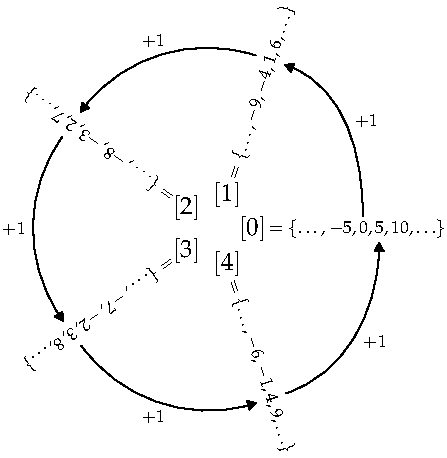
\includegraphics[scale=0.85]{cyclic-zn}%\\
			%Adding 1 in $\Z_5$\phantom{bo}
		\end{tabular}
	\end{minipage}%\vspace{-5pt}
\end{example}


\begin{thm}{}{zncyclic}
	$\Z_n$ forms an abelian group of order $n$ under addition modulo $n$.
\end{thm}

A rigorous proof (in the language of Footnote \ref{fn:eqclass}) is tedious, but will come for free in Chapter \ref{chap:coset} when $\Z_n$ is properly defined as a \emph{factor group.} These groups are so common that we usually just state ``The group $\Z_n$,'' rather than $(\Z_n,+_n)$. 
In the exercises, we'll also consider how \emph{multiplication} modulo $n$ can be used to create groups of remainders.

\goodbreak


\begin{examples}{}{}
	Here are the Cayley tables for $\Z_1,\Z_2,\Z_3$ and $\Z_4$.
	\[
		\begin{array}[t]{c||c}
			+_1 & 0\\\hline\hline
			0 & 0
		\end{array}
		\qquad
		\begin{array}[t]{c||c|c}
			+_2 & 0 & 1\\\hline\hline
			0 & 0 & 1\\\hline
			1 & 1 & 0
		\end{array}
		\qquad
		\begin{array}[t]{c||c|c|c}
			+_3 & 0 & 1 & 2\\\hline\hline
			0 & 0 & 1 & 2\\\hline
			1 & 1 & 2 & 0\\\hline
			2 & 2 & 0 & 1
		\end{array}
		\qquad
		\begin{array}[t]{c||c|c|c|c}
			+_4 & 0 & 1 & 2 & 3\\\hline\hline
			0 & 0 & 1 & 2 & 3\\\hline
			1 & 1 & 2 & 3 & 0\\\hline
			2 & 2 & 3 & 0 & 1\\\hline
			3 & 3 & 0 & 1 & 2
		\end{array}
	\]
	In each case 0 is the identity element. If you compare these to the the tables in  Example \ref*{ex:rx}.\ref{ex:smallcayley1}, the patterns should look familiar (we will explore this further in Section \ref{sec:morph}).
\end{examples}

\boldsubsubsection{Subgroups of $\Z_n$}

It is easy to spot certain subgroups of $\Z_n$ --- just think about divisors of $n$!

\begin{example}{}{z4subgroup}
	Plainly 2 is a divisor of 4. By covering up the rows/columns corresponding to 1 and 3, we obtain the  Cayley table for the subgroup $H=\{0,2\}$ of $\Z_4$. 
	\[
		\begin{array}[t]{c||c|c|c|c}
			+_4 & 0 & 1 & 2 & 3\\\hline\hline
			0 & 0 & 1 & 2 & 3\\\hline
			1 & 1 & 2 & 3 & 0\\\hline
			2 & 2 & 3 & 0 & 1\\\hline
			3 & 3 & 0 & 1 & 2
		\end{array}
		\quad
		\begin{array}[t]{c}
			\\
			\longrightarrow
		\end{array}
		\quad
		\begin{array}[t]{c||c|c}
			+_4 & 0 & 2\\\hline\hline
			0 & 0 & 2\\\hline
			2 & 2 & 0
		\end{array}
	\]
	Hopefully it is obvious why $H$ is a subgroup (think about the subgroup criterion Theorem \ref{thm:subgroup}!). Now suppose 1 were in some subgroup $K\le \Z_4$ and consider what the group axioms tell us:
	\begin{minipage}[t]{0.9\linewidth}\vspace{-6pt}
		\[
			\left.
			\begin{array}{ll}
				\text{Closure}&\Longrightarrow 2=1+1\in K\\
		  	\text{Inverse}&\Longrightarrow 3=-1\in K\\
		  	\text{Identity}&\Longrightarrow 0\in K
			\end{array}
			\right\}
			\implies K=\{0,1,2,3\}=\Z_4
		\]
		The same thing happens if a subgroup contains 3. The upshot is that $\Z_4$ has precisely three subgroups: itself, $\{0,2\}$ and the trivial subgroup $\{0\}$. The full subgroup diagram is drawn.
	\end{minipage}
	\hfill
	\begin{minipage}[t]{0.09\linewidth}\vspace{-5pt}
		\flushright$\xymatrix @R18pt{\Z_4 \ar@{-}[d]\\ \{0,2\} \ar@{-}[d]\\ \{0\}}$
	\end{minipage}
\end{example}

Here is a more general version. Suppose $d$ is a divisor of $n$, write $n=dk$, and consider the subset of \emph{multiples of $d$} in $\Z_n$:
\[
	\ip d=\bigl\{0,d,2d,\ldots,(k-1)d\bigr\}
\]
In the language of the subgroup criterion (Theorem \ref{thm:subgroup}), this set is:
\begin{quote}
	\begin{description}
		\item[Non-empty:] Plainly $0\in\ip d$.
		\item[Closed under addition:] $\kappa d+\lambda d=(\kappa+\lambda)d\in\ip d$.
		\item[Closed under inverses:] The inverse of $\lambda d$ is $-\lambda d=(k-\lambda)d\in\ip d$.
	\end{description}
\end{quote}

We have therefore proved:

\begin{lemm}{}{cyclicsg}
	If $d$ is a divisor of $n$, then the set of multiples $\ip{d}$ in $\Z_n$ is a subgroup of order $\frac nd$.
\end{lemm}

As in Example \ref{ex:z4subgroup}, in Chapter \ref{chap:cyclic} we'll see that these are in fact the \emph{only} subgroups of $\Z_n$.


\clearpage


\begin{exercises}
	Key concepts:\quad \emph{$\Z_n$,\quad Multiples as subgroups: $d\mid n\Longrightarrow \ip d\le\Z_n$}
	
	\begin{enumerate}
	  \item Refresh your memory of modular arithmetic by evaluating the following:
	  \begin{enumerate}
	    \item \makebox[200pt][l]{$17+22$ in $\Z_{30}$\hfill (b) }
	    	$31\cdot 4$ in $\Z_{12}$
	    	\setcounter{enumii}{2}
	    \item \makebox[200pt][l]{$5^6$ in $\Z_{14}$,\hfill (d) }
	    	$19^2-42\cdot 13$ in $\Z_{17}$
	  \end{enumerate}
	  
	  \item State the Cayley tables for the groups $\Z_5$ and $\Z_6$ (more formally $(\Z_5,+_5)$ and $(\Z_6,+_6)$).
	  
	  \item State the Cayley tables for all proper subgroups of $\Z_6$. Now draw the full subgroup diagram for $\Z_6$.\par
	  (\emph{Hint: consider Lemma \ref{lemm:cyclicsg} and the remark that follows})
	  
	  \item Draw the subgroup diagram for $\Z_{12}$.
	  	  
	 	\item Suppose $n$ is a positive integer $\ge 2$.
	  \begin{enumerate}
	    \item Explain why $\Z_n$ is \emph{not} a group under \emph{multiplication.} If you're unsure what to do, consider an example: what is the multiplication table for $(\Z_3,\cdot)$?	  
	  	\item Explain why $\{1,2,3,4,5\}$ isn't a group under multiplication modulo 6.
	   	\item Hypothesize for which integers $n\ge 2$ the set $\{1,2,3,\ldots,n-1\}$ forms a group under multiplication modulo $n$. If you want a challenge, try to prove your assertion.
	  \end{enumerate}
	  	  
	  \item\label{exs:znunits} The set $\Z_n^\times$ denotes the \emph{units} in $\Z_n$, those elements which are relatively prime to $n$:
	  \[
	  	\Z_n^\times=\bigl\{x\in\Z_n:\gcd(x,n)=1\bigr\}
	  \]
	  In part (d), we verify that $\Z_n^\times$ is an abelian group under multiplication modulo $n$.
	  \begin{enumerate}
	    \item Construct the Cayley tables for the groups $\Z_3^\times=\{1,2\}$ and $\Z_4^\times=\{1,3\}$.
	    \item\label{exs:z5times} Construct the Cayley table for the group $\Z_5^\times=\{1,2,3,4\}$. Now identify its \emph{subgroups.} 
	    \item\label{exs:znunits89} Construct the Cayley tables for $\Z_8^\times$ and $\Z_9^\times$. What is the order of each group?
	    \item (Hard)\lstsp Prove that $\Z_n^\times$ forms an abelian group under multiplication modulo $n$ by verifying the group axioms.\par
	    (\emph{Hint: Recall Bézout's identity $\gcd(x,n)=1\Longleftrightarrow\exists\kappa,\lambda\in\Z$ such that $\kappa x+\lambda n=1$})
	    \item\begin{enumerate}
	      \item Compare the orders of the groups $\Z_3^\times$, $\Z_4^\times$ and $\Z_{12}^\times$. What do you observe?
	      \item What about the orders of $\Z_2^\times$, $\Z_6^\times$ and $\Z_{12}^\times$? What is going on?
	      \item The order of $\Z_n^\times$ is the value of \emph{Euler's totient function} $\phi(n)$. Research some of the properties of this function: can you find something that helps explain your observations in parts i and ii? Better still, take a course in Number Theory!
	  	\end{enumerate}
	  	
	  \end{enumerate}
	    
	\end{enumerate}
\end{exercises}


\clearpage


\subsection{Geometric Symmetries \& Matrix Groups}\label{sec:geomgroups}

Geometric symmetries an matrices provide further large families of groups. 

Now consider any geometric figure that has some symmetry (typically viewed as rotational or reflective), such as a triangle, square, or tetrahedron. Each symmetry corresponds to a \emph{function} that transforms the original figure in such a way that the result occupies the same location as the original.

\begin{example}{Klein four-group}{klein4}
	The pictured rectangle has three obvious symmetries:\par
	\begin{minipage}[t]{0.65\linewidth}\vspace{0pt}
		 \begin{itemize}\itemsep2pt
		   \item[$(\textcolor{Green}{a})$] Rotation by \ang{180}.
		   \item[$(\textcolor{red}{b})$] Vertical reflection.
		   \item[$(\textcolor{blue}{c})$] Horizontal reflection.
		 \end{itemize}
	\end{minipage}
	\hfill
	\begin{minipage}[t]{0.34\linewidth}\vspace{-6pt}
		\flushright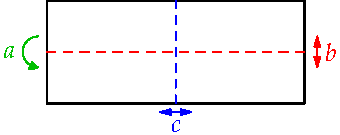
\includegraphics{group-klein2}
	\end{minipage}\par
	
	Each symmetry may be viewed as a function transforming the rectangle (or permuting its vertices/edges if you prefer). Group Theorists also consider the \emph{identity function} $e$ as a symmetry: it simply leaves the rectangle alone.\footnotemark{}\smallbreak
	It should be clear that the set $V:=\{e,a,b,c\}$ comprises every symmetry of the rectangle. We claim that $V$ forms a group whose binary operation is \emph{composition of functions.}\smallbreak
	\begin{description}
		\begin{minipage}[t]{0.8\linewidth}\vspace{-8pt}
			\item[Closure] After applying any two symmetries in sequence, the rectangle still occupies the same location on the page, the result of applying a \emph{single} symmetry.\par
				The composition table is shown and is easily be verified by, for instance, drawing a smiley face on one side of a sheet of paper.
		\end{minipage}
		\hfill
		\begin{minipage}[t]{0.19\linewidth}\vspace{-18pt}
			\flushright$\begin{array}[t]{c||c|c|c|c}
			\circ & e & \textcolor{Green}{a} & \textcolor{red}{b} & \textcolor{blue}{c}\\\hline\hline
			e & e & \textcolor{Green}{a} & \textcolor{red}{b} & \textcolor{blue}{c}\\\hline
			\textcolor{Green}{a} & \textcolor{Green}{a} & e & \textcolor{blue}{c} & \textcolor{red}{b}\\\hline
			\textcolor{red}{b} & \textcolor{red}{b} & \textcolor{blue}{c} & e & \textcolor{Green}{a}\\\hline
			\textcolor{blue}{c} & \textcolor{blue}{c} & \textcolor{red}{b} & \textcolor{Green}{a} & e
		\end{array}$
		\end{minipage}\par
		\vspace{-20pt}
		\begin{center}
			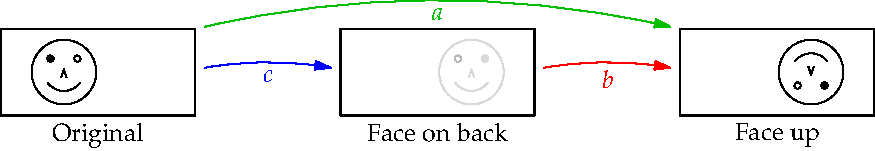
\includegraphics[scale=0.95]{group-klein3}\vspace{-15pt}
		\end{center}
		The pictures confirm $b\circ c=a$: remember that the \textbf{right side comes first} when composing functions! The diagonal symmetry of the table shows that the operation is \emph{commutative}.
		\item[Associativity] Composition of functions is always associative (Exercise \ref{exs:funcassoc}).
		\item[Identity] The function $e$ leaves the rectangle alone. Plainly $e\circ f=f\circ e=f$ for any symmetry $f$.
		\item[Inverse] To find the inverse of a symmetry, simply undo what you just did! In the case of the rectangle, every symmetry is its own inverse.
	\end{description}
	The symmetries of the rectangle thus form an abelian group of order 4. This is named the \emph{Klein four-group} in honor of Felix Klein, a 19\th{} century German mathematician whose application of group theory transformed modern geometry. The letter $V$ comes from the original German: \emph{vierergruppe.} 
\end{example}


\footnotetext{\label{fn:klein}%
	 There is little benefit to being explicit, but if you choose co-ordinates with the origin at the center of the rectangle, these functions can be written formulaically:
	\[
		e(x,y)=(x,y),\qquad a(x,y)=(-x,-y),\qquad b(x,y)=(x,-y),\qquad c(x,y)=(-x,y)
	\]%
}

\goodbreak


A similar discussion applies to any geometric figure.

\begin{thm}{}{rotationgroup}
	The \emph{symmetries} of any geometric figure form a group under composition.\smallbreak
	The \emph{orientation-preserving symmetries} form a subgroup, often called the \emph{rotation group}.\footnotemark{}
\end{thm}

\footnotetext{%
	In low dimensions, \emph{orientation-preserving} means that a transformation doesn't change the usual \emph{right-hand rule} (e.g., cross products). In two dimensions these are precisely the \emph{planar rotations}. In three dimensions a general orientation-preserving symmetry is the composition of two pure rotations (recall spherical polar co-ordinates).
}\vspace{-8pt}


\begin{example*}{\ref*{ex:subgroup2}.\ref{ex:circlegroup}, cont.}{}
	Since the complex function $z\mapsto e^{i\theta}z$ \emph{rotates} counter-clockwise by $\theta$ around the origin, the \emph{circle group} $S^1$ may be viewed as the group of rotations of the plane (or the circle).
\end{example*}

\begin{defn}{}{rot-dihedral}
	A regular $n$-gon has two commonly associated symmetry groups.%\vspace{-2pt}
	\begin{description}
	  \item[\emph{Dihedral Group}] The full symmetry group $D_n$ has order $2n$. It splits into two subsets of size $n$:
	  \begin{description}%\itemsep0pt
	    \item[\normalfont\emph{Rotations}] Labelled $e,\rho_1,\ldots,\rho_{n-1}$ where $\rho_k$ rotates counter-clockwise by $\frac{2\pi k}n$ radians ($\ang{\frac{360k}n}$). The identity $e=\rho_0$ is considered a rotation (by \ang 0).
	    \item[\normalfont\emph{Reflections}] These are typically labelled $\mu_k$ or $\delta_k$.
	  \end{description}
	  \item[\emph{Rotation group}] Denoted $R_n=\{e,\rho_1,\ldots,\rho_{n-1}\}$. This group is \emph{abelian,} which follows because composition of rotations simply sums angles:
	  \[
	  	\rho_j\circ\rho_k=\rho_{j+k\negthickspace\pmod n} =\rho_{k+j\negthickspace\pmod n} =\rho_k\circ\rho_j
	  \]
	\end{description}
\end{defn}


\begin{example}{}{d3}
	Denote the elements of the dihedral group $D_3$ as in the picture, where labeling the vertices 1, 2, 3 helps to keep track of things:\par
	\begin{minipage}{0.67\textwidth}\vspace{-5pt}
		\[
			D_3=\bigl\{e,\rho_1,\rho_2,\mu_1,\mu_2,\mu_3\bigr\}
		\]
		Its Cayley table is below. Constructing the table from scratch is a lot of work and is not worth memorizing!\smallbreak
		 The highlighted computation is $\textcolor{red}{\mu_1}\circ\textcolor{blue}{\rho_2}=\textcolor{Green}{\mu_3}$ (remember to 'do' $\textcolor{blue}{\rho_2}$ to the triangle first!). To verify, we could again try the smiley face trick, or alternatively consider the movement of a vertex:
		\begin{quote}
			$\textcolor{blue}{\rho_2}$ moves vertex 1 to vertex 3; $\textcolor{red}{\mu_1}$ moves this to vertex 2. Since the composition of a rotation and a reflection is a reflection (the triangle has been flipped over once!), the result must be the reflection mapping $1\mapsto 2$, namely $\textcolor{Green}{\mu_3}$.
		\end{quote}
		The lack of symmetry in the Cayley table shows that $D_3$ is a \emph{non-abelian group}: indeed
		\[
			\textcolor{blue}{\rho_2}\circ\textcolor{red}{\mu_1} =\mu_2\neq \textcolor{Green}{\mu_3}=\textcolor{red}{\mu_1}\circ\textcolor{blue}{\rho_2}
		\]
	\end{minipage}
	\hfill
	\begin{minipage}{0.32\textwidth}\vspace{-12pt}
		\flushright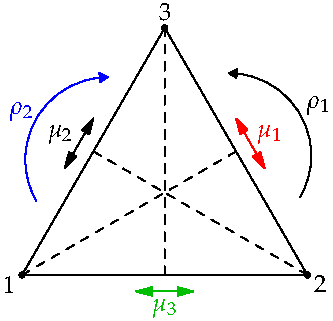
\includegraphics[scale=0.9]{group-d3}\smallbreak
		$\def\arraystretch{1.15}\begin{array}{c||c|c|c|c|c|c}
			\circ & e & \rho_1 & \textcolor{blue}{\rho_2} & \mu_1 & \mu_2 & \mu_3\\
			 \hline\hline
			e & e & \rho_1 & \rho_2 & \mu_1 & \mu_2 & \mu_3\\
			\hline
			\rho_1 & \rho_1 & \rho_2 & e & \mu_3 & \mu_1 & \mu_2\\
			\hline
			\rho_2 & \rho_2 & e & \rho_1 & \mu_2 & \mu_3 & \mu_1\\
			\hline
			\textcolor{red}{\mu_1} & \mu_1 & \mu_2 & \textcolor{Green}{\mu_3} & e & \rho_1 & \rho_2\\
			\hline
			\mu_2 & \mu_2 & \mu_3 & \mu_1 & \rho_2 & e & \rho_1\\
			\hline
			\mu_3 & \mu_3 & \mu_1 & \mu_2 & \rho_1 & \rho_2 & e
		\end{array}$
	\end{minipage}\bigbreak	
	\smash[b]{The Cayley table for the (abelian) rotation group $R_3=\{e,\rho_1,\rho_2\}$ is visible in the top left corner.}
\end{example}


\pagebreak


\boldsubsubsection{Geometric Subgroup Relations}

These are often straightforward to observe by drawing two shapes in such a way that all the symmetries of one are also symmetries of the other. Since the symmetries of both shapes form a group, this pictorial approach justifies the only necessary condition in Definition \ref{defn:subgroup}: the subset property.

\begin{examples}{}{hexsubgroup}
	\exstart For any $n$, we see that $R_n< S^1$: every rotation of a regular $n$-gon is also a rotation of a circle (with the same center).
	\begin{enumerate}\setcounter{enumi}{1}
	  \item\label{ex:hexsubgroup2} Consider a \textcolor{blue}{regular hexagon}, inside which have been drawn two \textcolor{red}{equilateral triangles}. Every symmetry of either triangle is also a symmetry the hexagon. We conclude:
	 	\begin{center}
			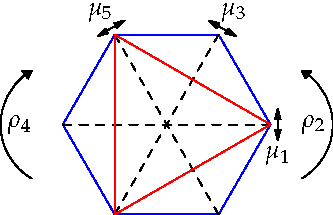
\includegraphics[scale=0.9]{group-hexagon3}
			\qquad\qquad
			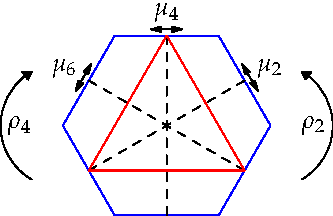
\includegraphics[scale=0.9]{group-hexagon4}
		\end{center}
	  \begin{enumerate}
	    \item $R_3< R_6$. Be careful with notation! With respect to the hexagon, $\rho_k$ is rotation counter-clockwise by $\ang{60k}$, whence the subgroup relation should be written 
	    \[
	    	R_3=\{e,\rho_2,\rho_4\} < R_6=\{e,\rho_1,\rho_2,\rho_3,\rho_4,\rho_5\}
	    \]
	    Also note that \emph{both triangles have the same rotation group.}
	    
	  	\item $D_3< D_6$. This is a little more complicated. Labeling the reflections $\mu_1,\ldots,\mu_6$ as in the picture, we see that the two triangles actually have different (full) symmetry groups:
			\[
				D_3^I=\{e,\rho_2,\rho_4,\mu_1,\mu_3,\mu_5\} < D_6
				\quad\text{and}\quad
				D_3^{II}=\{e,\rho_2,\rho_4,\mu_2,\mu_4,\mu_6\} < D_6
			\]
			Otherwise said, $D_6$ has two \emph{distinct} subgroups that look like $D_3$.
		\end{enumerate}
	\end{enumerate}
\end{examples}


\boldsubsubsection{Matrix Groups}

As observed in any elementary linear algebra course (see also Exercise \ref{exs:matrixassoc}), \textbf{matrix multiplication is associative}. This quickly yields several examples.

\begin{example}{}{gln}
	The \emph{general linear group} comprises the invertible $n\times n$ matrices under multiplication. For this course, only such matrices with real number entries will be encountered:
	\[
		\rGL_n(\R)=\bigl\{A\in \rM_n(\R):\det A\neq 0\bigr\} \tag{non-abelian when $n\ge 2$}
	\]
	\begin{minipage}[t]{0.8\linewidth}\vspace{-5pt}
		Since \textbf{associativity} holds in general, we need only verify the other three axioms.\smallbreak
		\textbf{Closure} follows from the familiar result $\det AB=\det A\det B$.\smallbreak
		The \textbf{identity} (drum roll\ldots) is the \emph{identity matrix} $I$.\smallbreak
		Finally, \textbf{invertibility} is assumed. Part 3 of Theorem \ref{thm:canc} should now seem very familiar: $(xy)^{-1}=y^{-1}x^{-1}$.
	\end{minipage}
	\hfill
	\begin{minipage}[t]{0.19\linewidth}\vspace{28pt}
		\flushright$I=\smash{\scalebox{0.8}{%
		$\begin{pmatrix}
			1&0&&\\
			0&1&\ddots&\\
			&\ddots&\ddots&0\\
			&&0&1
		\end{pmatrix}$%
		}}$
	\end{minipage}
\end{example}


\goodbreak


\boldsubsubsection{Matrix subgroups}

The general linear group $\rGL_n(\R)$ has many subgroups. Here is one; some others are in the Exercises.

\begin{example}{}{orthogonal}
The \emph{orthogonal group} $\rO_n(\R)=\{A\in\rM_n(\R):A^TA=I\}$ consists of those matrices whose inverse equals their transpose ($A^{-1}=A^T$). We verify that this is a subgroup of $\rGL_n(\R)$ using the subgroup criterion (Theorem \ref{thm:subgroup}) and simple matrix properties.
	\begin{description}
	  \item[Non-empty subset] Every orthogonal matrix is invertible, whence $\rO_n(\R)\subseteq\rGL_n(\R)$. This is immediate in two ways: if $A\in\rO_n(\R)$, then,
	  \begin{gather*}
	  	A^TA=I\implies A^{-1}=A^T \text{ exists, \ or,}\\
	  	1=\det I=\det A\det A^T=(\det A)^2\implies \det A\neq 0
	  \end{gather*}
	  Moreover, $I^TI=I^2=I$, so $I\in\rO_n(\R)$: we have non-emptiness.
	  \item[Closure] Suppose $A,B\in\rO_n(\R)$. Then
	  \begin{gather*}
	  	(AB)^T(AB)=B^TA^TAB=B^TIB=B^TB=I \implies AB\in\rO_n(\R)
	  \end{gather*}
	  \item[Inverses] Suppose $A\in\rO_n(\R)$. Then
	  \begin{gather*}
	  	(A^{-1})^TA^{-1}=(A^T)^TA^T=(AA^T)^T=I^T=I\implies A^{-1}\in\rO_n(\R)
	  \end{gather*}
	\end{description}
	The $2\times 2$ orthogonal matrices can be interpreted as rotations and reflections.\footnotemark{} For instance, the matrix $\frac 1{\sqrt 2}
	\begin{smatrix}
		1&-1\\
		1&1
	\end{smatrix}
	\in\rO_2(\R)$ rotates the plane counter-clockwise by \ang{45}.
\end{example}

\footnotetext{\label{fn:o2matrices}%
	You might have seen this in another course. Left-multiplication by:
	\begin{itemize}
		\item $\begin{smatrix}
			\cos\theta&-\sin\theta\\
			\sin\theta&\cos\theta
		\end{smatrix}$ rotates vectors counter-clockwise by $\theta$ radians.
		\item $\begin{smatrix}
			\cos\theta&\sin\theta\\
			\sin\theta&-\cos\theta
		\end{smatrix}$
		reflects across the line making angle $\theta/2$ with the positive real axis.
	\end{itemize}
	This interpretation allows us to view $D_n$ as a subgroup of $\rO_2(\R)$.
}


\vfil


\begin{exercises}
	Key concepts:\quad \emph{Klein 4-group $V$\quad Dihedral group $D_n$\quad Rotation group $R_n$}
	\begin{quote}
		\emph{Geometric subgroup relations\quad General linear group $\rGL_n(\R)$}
	\end{quote}

	\begin{enumerate}
	 	\item Use Theorem \ref{thm:subgroup} to explain why the set of \emph{rotations} of a planar figure is a subgroup of its full symmetry group (rotations \emph{and} reflections).
	  
	  
	  \item\label{exs:squarerot} Explicitly state the Cayley table for the rotation group $R_4$ of a square.

	  
	  \item Find the subgroup diagram of the Klein four-group. Explain how you know you are correct.
	  
	  
	  \item Repeat the previous question for the rotation group $R_6$. 

		
		\item\begin{enumerate}
		  \item Find all subgroups and the subgroup diagram for the group $D_3$.\par
		  (Don't worry about being rigorous as to how you know you've found them all.)
	    \item Describe the symmetry group and Cayley table of a \emph{non-equilateral} isosceles triangle. What about a \emph{scalene} triangle?
		\end{enumerate}
		
				
	  \goodbreak
	  

	  \item\begin{enumerate}
	    \item Represent the elements of the Klein four-group $V$ (as in Footnote \ref{fn:klein}) using matrix notation (i.e. $a$ is left-multiplication by what matrix). As such, identify $V$ as a subgroup of $\rO_2(\R)$.
	    \item Modeling Example \ref{ex:hexsubgroup}, draw three pictures which describe different ways in which $V$ may be viewed as a subgroup of $D_6$.
	  \end{enumerate}
	  
	  
	  \item Determine whether each of the following sets of matrices is a group under multiplication.
	  \begin{enumerate}
	    \item \makebox[210pt]{$\mathcal K=\{A\in \rM_2(\R):\det A=\pm 1\}$\hfill (b)\lstsp} $\mathcal L=\{A\in \rM_2(\R):\det A=7\}$\setcounter{enumii}{2}
	    
	    \item $\mathcal N=\bigl\{\begin{smatrix}
	    a&b\\0&d
	    \end{smatrix}\in\rM_2(\R):ad\neq 0\bigr\}$
	  \end{enumerate}
	  
	  
	  \item\label{exs:subgpmatrix} Prove that each set of matrices forms a group under multiplication (don't memorize these---unless you really love matrices\ldots).
	  \begin{enumerate}
	    \item Special linear group: $\rSL_n(\R)=\bigl\{A\in \rM_n(\R):\det A=1\bigr\}$
	    
	    \item Special orthogonal group: $\rSO_n(\R)=\{A\in\rM_n(\R):A^TA=I\text{ and }\det A=1\}$
	    
	    \item $\mathcal Q_n=\bigl\{A\in \rM_n(\R):\det A\in\Q^\times\bigr\}$
	    
% 	    \item (Harder)\lstsp Symplectic group: $\rSp_{2n}(\R)=\bigl\{A\in \rM_{2n}(\R):A^TJA=J\bigr\}$, where $J=\scalebox{0.6}{$\left(\!
% 	    \begin{array}{c|c}
% 	    	0&I_n\\
% 	    	\hline -I_n&0
% 	    \end{array}
% 	    \!\right)$}$ is a block matrix and $I_n$ the $n\times n$ identity matrix.
	    
	    \item (Hard)\lstsp $\rSL_n(\Z)=\bigl\{A\in \rM_n(\Z):\det A=1\bigr\}$: all entries in these matrices are \emph{integers.}\par
	    (\emph{Hint: look up the classical adjoint $\operatorname{adj}A$ of a square matrix})
	  \end{enumerate}
	  Now construct a diagram showing the subgroup relationships between the groups
	  \[
	  	\rGL_n(\R),\quad \rSL_n(\R),\quad \rO_n(\R),\quad \rSO_n(\R),\quad \mathcal Q_n,\quad \rSL_n(\Z)
	  \]

		\item\label{exs:funcassoc}
		\begin{enumerate}
		  \item Let $X$ be any set. Prove that composition of functions $f:X\to X$ is associative.\par
			(\emph{Hint: $(f\circ g)\circ h=f\circ(g\circ h)$ means that both functions do the same thing to the same input\ldots})
			\item Suppose $X$ contains at least two distinct elements $a\neq b$. Prove that there exist functions $f,g:X\to X$ for which $f\circ g\neq g\circ f$.
		\end{enumerate}

	  
	  \item\label{exs:matrixassoc}\begin{enumerate}
			\item Prove that matrix multiplication of (real square) matrices is associative.\par
		(\emph{Hint: If $A$ has entries $(a_{ij})$, etc., what are the $pq\th$ entries of the matrices $A(BC)$ and $(AB)C$?})
			\item Show that multiplication of (invertible) $n\times n$ matrices is non-commutative when $n\ge 2$.
		\end{enumerate}


		\item Prove that $D_n$ is non-abelian ($n\ge 3$).\par
		(\emph{Hint: label vertices and proceed as is Example \ref{ex:d3}})
	
	  

	  \begin{minipage}[t]{0.69\linewidth}\vspace{0pt}
	    \item\label{exs:dnddice} Consider rotating (in 3D) a regular \textcolor{blue}{tetrahedron}. Any face (equilateral triangle) may be rotated to its desired location (four options), in which it has three possible orientations. The rotation group of the tetrahedron therefore has $4\times 3=12$ elements.
	  	\begin{enumerate}\itemsep0pt
	    	\item Find the order of the rotation group of a \textcolor{orange}{cube}.
	    	\item Repeat for a regular \textcolor{Green}{octahedron}. Give a \emph{geometric} reason why your answer is the same as part (a).\par
	    	(\emph{Hint: Try joining the midpoints of each face\ldots}).
	    	\item What about the \textcolor{Goldenrod}{dodecahedron} and the \textcolor{violet}{icosahedron}?!
	  	\end{enumerate}
	    \end{minipage}
	    \hfill
	   	\begin{minipage}[t]{0.29\linewidth}\vspace{0pt}
	  		\flushright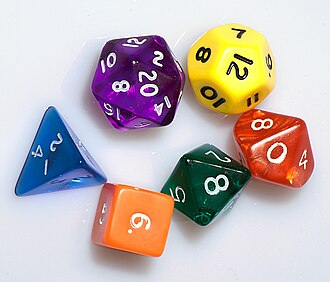
\includegraphics[scale=0.4]{groups-dice}\par
	  		\centering Common polyhedral dice
	    \end{minipage}\medbreak
	    In case you don't recognize it, the pictured \textcolor{red}{red die} is not one of the five Platonic solids: it has ten rhombus-shaped faces, and its rotation group has order 10. We'll return to these examples in later sections.
	  
	\end{enumerate}
\end{exercises}


\clearpage


\subsection{Homomorphisms \& Isomorphisms}\label{sec:morph}

In the previous sections, you should have felt like you were encountering similar examples in different contexts. A key goal of abstract mathematics is the comparison of similar/identical structures with outwardly different appearances. The standard approach to such comparison is uses \emph{functions.}

\begin{example}{}{z3r3iso}
	Compare the rotation group $R_3$ of an equilateral triangle to the modular arithmetic group $\Z_3$. Their Cayley tables look almost identical, particularly if we write $\rho_0$ for the identity in $R_3$. To a mathematician, the groups have the same \emph{structure}; they are merely labelled differently.\par
	\begin{minipage}[t]{0.63\linewidth}\vspace{-5pt}
		\emph{Relabelling} means defining an \emph{invertible function} $\mu:R_3\to \Z_3$: the obvious choice from looking at the tables is $\mu(\rho_k)=k$.\smallbreak
		Since the tables describe all possible interactions between the elements of each group, it is clear that $\mu$ satisfies
		\[
			\forall \rho_j,\rho_k\in R_3,\ \ \mu(\rho_j\circ\rho_k)=\mu(\rho_j)+_3\mu(\rho_k)
		\]
	\end{minipage}
	\hfill
	\begin{minipage}[t]{0.36\linewidth}\vspace{-8pt}
		\flushright\def\arraystretch{1.5}
		\begin{tabular}{@{}cc@{}}\def\arraystretch{1}
			$\begin{array}[t]{c||c|c|c}
				\circ&\rho_{\textcolor{red}{0}}&\rho_{\textcolor{blue}{1}}&\rho_{\textcolor{Green}{2}}\\\hline\hline
				\rho_{\textcolor{red}{0}}&\rho_{\textcolor{red}{0}}&\rho_{\textcolor{blue}{1}}&\rho_{\textcolor{Green}{2}}\\\hline
				\rho_{\textcolor{blue}{1}}&\rho_{\textcolor{blue}{1}}&\rho_{\textcolor{Green}{2}}&\rho_{\textcolor{red}{0}}\\\hline
				\rho_{\textcolor{Green}{2}}&\rho_{\textcolor{Green}{2}}&\rho_{\textcolor{red}{0}}&\rho_{\textcolor{blue}{1}}
			\end{array}$
			&\def\arraystretch{1}
			$\begin{array}[t]{c||c|c|c}
				+_3&\textcolor{red}{0}&\textcolor{blue}{1}&\textcolor{Green}{2}\\\hline\hline
				\textcolor{red}{0}&\textcolor{red}{0}&\textcolor{blue}{1}&\textcolor{Green}{2}\\\hline
				\textcolor{blue}{1}&\textcolor{blue}{1}&\textcolor{Green}{2}&\textcolor{red}{0}\\\hline
				\textcolor{Green}{2}&\textcolor{Green}{2}&\textcolor{red}{0}&\textcolor{blue}{1}
			\end{array}$\\
			$(R_3,\circ)$
			&
			$(\Z_3,+_3)$
		\end{tabular}
	\end{minipage}\bigbreak
	Indeed, both sides simply equal $j+_3k$! This is a critical formula. To see why, suppose we are given remainders $x,y\in\Z_3$ and consider two courses of action:
	\begin{enumerate}\itemsep2pt
	  \item \emph{First combine} the remainders $x+_3y$ in $\Z_3$, \emph{then map} to $R_3$ using the function to obtain $\mu(x+_3y)$.
	  \item \emph{First map} both remainders to $R_3$ using $\mu$, \emph{then combine} in $R_3$ to obtain $\mu(x)\circ\mu(y)$.
	\end{enumerate}
	Regardless of the order (combine/map or map/combine) \emph{we always obtain the same result}! Such \emph{structure-preserving functions} are at the heart of abstract algebra.
\end{example}


\begin{defn}{Homo- \& Isomorphisms}{homoiso}
	Suppose $(G,\ast)$ and $(H,\star)$ are binary structures and $\phi:G\to H$ a function. We say that $\phi$ is a \emph{homomorphism} of binary structures if
	\[
		\forall x,y\in G,\ \ \phi(x\opast y)=\phi(x)\opstar\phi(y)
	\]
	An \emph{isomorphism}\footnotemark{} of binary structures $G,H$ is a \emph{bijective/invertible homomorphism} $\mu:G\to H$.\smallbreak
	Binary structures $G,H$ are \emph{isomorphic}, written $G\cong H$, if there exists some isomorphism $\mu:G\to H$. 
\end{defn}

\footnotetext{%
	These terms come from ancient Greek: \emph{homo-} (similar, alike), \emph{iso-} (equal, identical), and \emph{morph(e)} (shape, structure).%
}

The notation is typical: $\mu$ (rather than $\phi$) is often used when we know we have an \emph{iso}morphism. For most of these notes (certainly after this chapter), all binary structures will be groups.


\begin{examples}{}{}
	\exstart (\ref{ex:z3r3iso} cont.)\quad 	We have \emph{isomorphic groups} $R_3\cong\Z_3$. Indeed the function $\mu:R_3\to\Z_3$ is an \emph{isomorphism of groups} (or \emph{group isomorphism}).
	
	\begin{enumerate}\setcounter{enumi}{1}
	  \item The%
		\def\opbl{\mathbin{\textcolor{blue}{+}}}
		\def\oprd{\mathbin{\textcolor{red}{+}}} 
		function $\phi:(\N,\textcolor{red}{+})\to(\R,\textcolor{blue}{+})$ defined by $\phi(x)=\sqrt 2x$ is a homomorphism (of binary structures: $(\N,+)$ is not a group!),
		\[
			\phi(x\oprd y)=\sqrt 2(x\oprd y)=\sqrt 2x\opbl \sqrt 2y=\phi(x)\opbl \phi(y)
		\]
		As before, it is worth spelling this out:
		\begin{quote}
	  	\emph{Sum then map} $\phi(x\oprd y)$ gives the same result as \emph{map then sum} $\phi(x)\opbl\phi(y)$.
		\end{quote}
		
		
		\goodbreak
		
		
	  \item If $V,W$ are vector spaces then every linear map $\rT:V\to W$ is a group homomorphism:\footnotemark
	  \[
	  	\forall\vv_1,\vv_2\in V,\quad \rT(\vv_1+\vv_2)=\rT(\vv_1)+\rT(\vv_2)
	  \]
	  You've been encountering homomorphisms your entire mathematical career: for instance, both the calculus identity $\diff x(f+g)=\diff[f]{x}+\diff[g]{x}$ and the distributive law of matrix multiplication $A(\vx+\vy)=A\vx+A\vy$ are homomorphism properties! 
	  
	  \item (\emph{Trivial homomorphism})\lstsp If $G$ and $L$ are any groups, then the function $\phi:G\to L$ defined by $\phi(g)=e_L$ (the identity in $L$) is a homomorphism:
	  \[
	  	\forall x,y\in G,\ \ \phi(xy)=e_L=(e_L)^2=\phi(x)\phi(y)
	  \]
	  
	  \item (\emph{Inclusion map})\lstsp If $H$ is a subgroup of $G$, then $\phi(x)=x$ defines a homomorphism $\phi:H\to G$:
	  \[
	  	\forall x,y\in G,\ \ \phi(xy)=xy=\phi(x)\phi(y)
	  \]
	  
	  \item\def\3nth{\negthickspace\negthickspace\negthickspace} The function $\phi(\rho_k)=\rho_{2k\negthickspace\pmod 4}$ is a homomorphism $\phi:R_4\to R_4$:
	  \begin{align*}
	  	\phi(\rho_j\circ\rho_k)&=\phi(\rho_{j+k\3nth\pmod 4}) 
	  	=\rho_{2(j+k)\3nth\pmod 4} =\rho_{2j\3nth\pmod 4}\circ \rho_{2k\3nth\pmod 4}\\
	  	&=\phi(\rho_j)\circ\phi(\rho_k)	  
	  \end{align*}
	\end{enumerate}
\end{examples}

\footnotetext{%
	The scalar multiplication condition $\rT(\lambda\vv)=\lambda \rT(\vv)$ of a linear map is not relevant here.%
}
\vspace{-5pt}

\boldsubsubsection{Establishing Isomorphicity}

We must do four things if we suspect binary structures $(G,*)$ and $(H,\star)$ to be isomorphic:
\begin{quote}
	\begin{description}
		\item[\emph{Definition}:] Define $\mu:G\to H$ and, if necessary, verify that it is a function.\footnote{%
			If $G$ is a set of equivalence classes, we also need to check that $\phi$ is \emph{well-defined.} This subtlety is why we haven't (yet) had an example where $\Z_n$ is the \emph{domain} of a homomorphism. We will do so later (Example \ref*{ex:unisoex}.\ref{ex:unisoex2}, Theorem \ref{thm:cyclicisomorph}, etc.).
			}
		\item[\emph{Homomorphism}:] Verify that $\mu(x\opast y)=\mu(x)\opstar\mu(y)$ for all $x,y\in G$.
		\item[\emph{Injectivity/1--1}:] Check that $\mu(x)=\mu(y)\Longrightarrow x=y$.
		\item[\emph{Surjectivity/onto}:] Check $\operatorname{range}\mu=H$. Equivalently $\forall h\in H,\ \exists g\in G$ such that $h=\mu(g)$.
	\end{description}
\end{quote}

The last three steps can be done in any order, and injectivity/surjectivity can be combined if you manage to exhibit an explicit \emph{inverse function} $\mu^{-1}:H\to G$. If you are unsure how to start, often the best thing is to play with the homomorphism property itself.


\begin{examples}{}{expiso}
	\exstart We show that $(2\Z,+)$ and $(3\Z,+)$ are isomorphic groups.
	\begin{enumerate}\setcounter{enumi}{1}
	  \item[]\begin{description}
	  	\item[\emph{Definition}:] The obvious candidate\footnotemark{} is $\phi(x)=\frac 32x$. Plainly $\phi(2n)=3n$ whence $\phi:2\Z\to 3\Z$.
	  	\item[\emph{Homomorphism}:] $\phi(x+y)=\frac 32(x+y)=\frac 32x+\frac 32y=\phi(x)+\phi(y)$
	  	\item[\emph{Injectivity}:] $\phi(x)=\phi(y)\Longrightarrow \frac 32x=\frac 32y\Longrightarrow x=y$.
	  	\item[\emph{Surjectivity}:] If $z=3n\in 3\Z$, then $z=\frac 32\cdot\frac 23z=\frac 32(2n)=\phi(2n)\in\operatorname{range}\phi$.
		\end{description}
		The last steps are essentially the observation that $\phi^{-1}(z)=\frac 23z$.\smallbreak
		More generally, the groups $(m\Z,+)$ and $(n\Z,+)$ are isomorphic whenever $m,n\neq 0$. 
	
		\item\label{ex:expiso1}	We prove that $(\R,+)\cong(\R^+,\cdot)$: these are isomorphic abelian groups (recall that $\R^+=(0,\infty)$ is the set of \emph{positive real numbers}).
		\begin{description}
	  	\item[\emph{Definition}/\emph{Homomorphism}:] We need a bijective function $\mu:\R\to\R^+$ which converts addition to multiplication $\mu(x+y)=\mu(x)\mu(y)$. But \emph{exponentiation} does exactly this: defining $\mu(x)=e^x$, we see that the homomorphism property is the familiar exponential law! 
	  	\[
	  		\mu(x+y)=e^{x+y}=e^xe^y=\mu(x)\mu(y)
	  	\]
	  	\item[\emph{Bijectivity}:] $\mu^{-1}(z)=\ln z$ is the inverse function of $\mu$.
		\end{description}
		Other exponential functions also provide suitable isomorphisms: e.g.{} $2^x,10^x$, etc.
	\end{enumerate}
\end{examples}

\footnotetext{%
	You might think, ``How can I turn an even number into a multiple of three?'' Of perhaps you start by thinking about the homomorphism property: multiplication by a constant certainly satisfies $\phi(x+y)=\phi(x)+\phi(y)$.%
}



\boldsubsubsection{Demonstrating Non-Isomorphicity (Structural Properties)}

Suppose we suspect that binary structures $(G,*)$ and $(H,\star)$ are non-isomorphic. Unless $G,H$ are very small, individually verifying that every possible function $\mu:G\to H$ is a non-isomorphism would be unrealistic! Instead we consider \emph{structural properties}: properties that isomorphic structures must share. If any such is held by one structure but not the other, then the structures are non-isomorphic.\smallbreak

Here is a non-exhaustive list of structural properties; we'll check some in Exercise \ref{exs:structural1}. Throughout, we assume that $\mu:(G,*)\to (H,\star)$ is an isomorphism. 
\begin{description}\itemsep0pt
  \item[\emph{Cardinality/order}:] Since $G$ and $H$ are bijectively paired, their cardinalities are the same.
  \item[\emph{Commutativity \& Associativity}:] Suppose $(G,\ast)$ is commutative and let $X,Y\in H$. Since $\mu$ is surjective, we may write $X=\mu(x)$ and $Y=\mu(y)$ for some $x,y\in G$. The homomorphism property now shows that $(H,\star)$ is commutative:
  \[
  	X\opstar Y=\mu(x)\opstar\mu(y) =\mu(x\opast y) =\mu(y\opast x) =\mu(y)\opstar\mu(x) =Y\opstar X
  \]
  The argument for associativity is similar, though more tedious.
  \item[\emph{Identities \& Inverses}:] If $(G,\ast)$ has identity $e$, then $\mu(e)$ is the identity for $(H,\star)$. Similarly $\mu$ maps inverses to inverses.
  \item[\emph{Solutions to equations}:] Related equations have the same number of solutions. For instance,
  \[
  	x\opast x=x\iff \mu(x)\opstar\mu(x)=\mu(x)
  \]
  says that the equations $x\opast x=x$ (in $G$) and $z\opstar z=z$ (in $H$) have the same number of solutions.\footnotemark
  \item[\emph{Being a group}] If $G$ is a group, so also is $H$.
\end{description}

\footnotetext{%
	Such solutions are called \emph{idempotents}; thus existence of idempotents is itself a structural property.%
}



\begin{examples}{}{}
	\exstart Recall that $\N_0=\{0,1,2,3,\ldots\}$. Since $(\N_0,+)$ contains the identity element 0 whereas $(\N,+)$ has no identity, we conclude that these binary structures are non-isomorphic.

	\begin{enumerate}\setcounter{enumi}{1}%\itemsep2pt
	  \item $\Z_5$ is not isomorphic to $D_3$ since the two groups have different orders (5 and 6).
	  
	  \goodbreak
	  
	  \begin{minipage}[t]{0.72\linewidth}\vspace{0pt}
	  	\item The binary structures defined by the two tables are non-isomorphic. For instance, the first is commutative while the second is not.
	  		  
	  	\item $\rGL_2(\R)$ and $(\R,+)$ are non-isomorphic for the same reason: the first is non-abelian and the second abelian.
	  \end{minipage}
	  \hfill
	  \begin{minipage}[t]{0.27\linewidth}\vspace{0pt}
		  \flushright%
		  $\begin{array}[t]{c||c|c}
				* & a & b\\
				\hline\hline a & a & b\\
				\hline b & b & a
		  \end{array}
		  \quad
		  \begin{array}[t]{c||c|c}
				\star & c & d\\
				\hline\hline c & c & d\\
				\hline d & c & d
		  \end{array}$
	  \end{minipage}
	  \par 
	 	
 	  %\item The groups $(\Z_6,+_6)$ and $D_3$ both have order six, but are non-isomorphic since $\Z_6$ is abelian and $D_3$ is not
	  
	  \item To see that $(\Q,+)$ and $(\R,+)$ are non-isomorphic groups, it is enough to recall that the sets have different cardinalities: $\Q$ is \emph{countably infinite} while $\R$ is \emph{uncountable.}


		\item The groups $(\Z,+)$ and $(\Q,+)$ have the same (countably infinite) order, and are both abelian. To see that they are non-isomorphic, consider the equation $x+x=1$ which has no solutions in $\Z$. If $\mu:\Z\to\Q$ were an isomorphism, then the equation $\mu(x)+\mu(x)=\mu(1)$ does have a solution $y=\mu(x)=\frac 12\mu(1)$ in $\Q$. But then $x=\mu^{-1}(y)$ solves the original equation: contradiction!
 	  
 	  
 	  \item $(S^1,\cdot)$ and $(\R,+)$ are non-isomorphic: consider the equations $x*x=e$\ldots
	\end{enumerate}
\end{examples}

Many properties are non-structural and therefore \emph{cannot} be used to show non-isomorphicity: the type of element (number, matrix, etc.), the type of binary operation (addition, multiplication, etc.).



\boldsubsubsection{Transferring a Binary Structure}

Suppose $\mu:G\to H$ is a bijection of \emph{sets}, where one of $G,H$ has a binary structure. A binary structure may be \emph{defined} on the other by insisting that $\mu$ be an isomorphism.

\begin{example}{}{pull-back}
% \exstart As already seen, $\phi:2\Z\to3\Z:x\mapsto\frac 32x$ is a bijection. Define $\star$ on $3\Z$ by
% \[w\opstar z:=\frac 13wz \tag{$3m\opstar 3n=\frac 13(3m)(3n)=3mn\in 3\Z$}\]
% The pull-back of $\star$ to $2\Z$ is then
% \[x\opast y= \frac 23\left(\frac 32 x\opstar\frac 32y \right) =\frac 23\cdot \frac 34xy=\frac 12xy\]
% which is easily confirmed to be a binary operation on $2\Z$. Since $\phi$ is an isomorphism, we can verify certain shared structural properties:
% \begin{quote}
% \begin{description}
%   \item[\normalfont\emph{Cardinality}:] $2\Z$ and $3\Z$ are both uncountably infinite sets.
%   \item[\normalfont\emph{Commutativity \& Associativity}:] Both are commutative and associative, e.g.
%   \[a\opast (b\opast c)=(a\opast b)\opast c=\frac 14abc\]
%   \item[\normalfont\emph{Identities}:] $(2\Z,\ast)$ has identity 2 (e.g.\ $2\opast x=\frac 12\cdot 2x=x$) and $(3\Z,\star)$ has identity $\phi(2)=3$.
%   \item[\normalfont\emph{Inverses}:] Neither has inverses and therefore neither is a group: e.g. $4\in 2\Z$ has no inverse
%   \[4\opast x=2\iff 2x=2\iff x=1\not\in 2\Z\]
% \end{description}
% \end{quote}
  The function $\mu(x)=x^3+8$ is a bijection $\R\to\R$. Starting with the binary (group) structure $(\R,+)$ and treating $\mu$ as an isomorphism, we may create a new isomorphic structure. There are two ways to do this:
  \begin{description}
  	\item[\emph{Pull-back}:] Suppose $\mu:(\R,*)\to (\R,+)$. Since $\mu(x\opast y)=\mu(x)+\mu(y)$, the new operation $\ast$ must be
			\[
				x\opast y:=\mu^{-1}\bigl(\mu(x)+\mu(y)\bigr) 
				=\mu^{-1}(x^3+y^3+16) 
				=\sqrt[3]{x^3+y^3+8}
			\]
			All structural properties transfer from $(\R,+)$ to $(\R,*)$: for instance, $(\R,*)$ is an abelian group with identity element
			\[
				\mu^{-1}(0)=\sqrt[3]{-8}=-2
			\]
			As a sanity check, observe that we really do have $x\opast (-2)=\sqrt[3]{x^3+(-2)^3+8}=x$!
			\item[\emph{Push-forward}:] View $\mu:(\R,+)\to (\R,*)$ as an isomorphism. Computation of $*$ is an exercise.
  \end{description} 
\end{example}




\boldsubsubsection{``Up to Isomorphism''}\phantomsection\label{sec:uptoiso} 

\begin{minipage}[t]{0.85\linewidth}\vspace{-10pt}
	This phrase is ubiquitous in group theory. To illustrate, consider that if $\bigl(\{e,a\},*\bigl)$ is a group with identity $e$, then its Cayley table must be as shown (Example \ref*{ex:rx}.\ref{ex:smallcayley1}). Otherwise said: there may be \emph{infinitely many distinct groups of order two, but all are isomorphic to each other.} This is too wordy, so a mathematician might instead say:
\end{minipage}
\hfill
\begin{minipage}[t]{0.14\linewidth}\vspace{-10pt}
	\flushright%
	$\begin{array}[t]{c||c|c}
		* & e & a\\\hline\hline
		e & e & a\\\hline
		a & a & e
	\end{array}$
\end{minipage}\par

\begin{quote}
	\emph{Up to isomorphism,} there is a unique group of order two.
\end{quote}
Make sure you include the snippet ``up to isomorphism,'' for otherwise the sentence is \emph{false}!


\goodbreak


The start of group theory can feel very challenging. With its focus on functions and its unfamiliar words, this last introductory section likely seems particularly so. Complete fluency with the vocabulary is \emph{not required} at this stage. The remaining chapters provide plenty opportunity to reinforce the language introduced in this chapter.\smallbreak
For the same reason, several of the following Exercises (particularly number \ref*{exs:structural1} onwards) will likely seem difficult. Try these (and discuss them) now, even if you aren't sure what to do; return later when you feel more comfortable. Learning abstract concepts isn't quick; give the ideas a chance to sink in. By the end of the course, these Exercises \emph{should} seem much easier!

\begin{exercises}{}
	Key concepts:\quad \emph{Homomorphism\quad Isomorphism\quad Injective/surjective/bijective}
	\begin{quote}
		\emph{Structural property\quad `Up to isomorphism'}
	\end{quote}
	
	\begin{enumerate}	  
		\item Which of the following are homomorphisms/isomorphisms of binary structures? Explain.
	  \begin{enumerate}
	    \item \makebox[210pt][l]{$\phi:(\Z,+)\to (\Z,+)$, \ $\phi(n)=-n$\hfill (b)\ }
	    $\phi:(\Z,+)\to (\Z,+)$, \ $\phi(n)=n+1$
	    \setcounter{enumii}{2}
	    
	    \item \makebox[210pt][l]{$\phi:(\Q,+)\to (\Q,+)$, \ $\phi(x)=\frac{4}{3}x$\hfill (d)\ }
	    $\phi:(\Q,\cdot)\to (\Q,\cdot)$, \ $\phi(x)=x^2$
	    \setcounter{enumii}{4}
	    
	    \item \makebox[210pt][l]{$\phi:(\R,\cdot)\to (\R,\cdot)$, \ $\phi(x)=x^5$\hfill (f)\ }
	    $\phi:(\R,+)\to (\R,\cdot)$, \ $\phi(x)=2^x$
	    \setcounter{enumii}{6}
	    
	    \item %\makebox[210pt][l]{$\phi:(R_4,\circ)\to (\Z_8,+_8)$, \ $\phi(\rho_k)=2k$\hfill (h)\ }
	    $\phi:(\rM_2(\R),\cdot)\to (\R,\cdot)$, \ $\phi(A)=\det A$
	    %\setcounter{enumii}{8}
	    
	    \item $\phi:(\rM_n(\R),+)\to (\R,+)$, $\phi(A)=\tr A$ \ (trace: add the entries on the main diagonal)
	  \end{enumerate}
	  
	  
	  \item Show that $(\Z,+)\cong (n\Z,+)$ for any \emph{non-zero} constant $n$.
	  
	  
% 	  \item In Example \ref{ex:z3r3iso} we saw that $R_3\cong \Z_3$ via the explicit isomorphism $\mu(\rho_k)=k$. Find a \emph{second} isomorphism $\psi:R_3\to\Z_3$.
	  
	  
	  \item Prove or disprove: $(\R^3,+)\cong(\R^3,\times)$ (cross product). 
	  
	  
	  \item $\mu(n)=2-n$ is a bijection of $\Z$ with itself. For each of the following, define a binary relation $*$ on $\Z$ such that $\mu$ is an isomorphism.
	  \begin{enumerate}
	    \item $\mu:(\Z,*)\to (\Z,+)$\quad\qquad
	    (b) \ $\mu:(\Z,*)\to (\Z,\cdot)$\quad\qquad 
	    (c) \ $\mu:(\Z,*)\to (\Z,\max(a,b))$
	  \end{enumerate}

	  
	  \item Finish Example \ref{ex:pull-back} by computing the push-forward $X\opast Y$ for any $X,Y\in \R$.
	  
	  
		\item $\mu(x)=x^2$ is a bijection $\mu:\R^+\to\R^+$. Find $x\opast y$ if $\mu$ is to be an isomorphism.
		\begin{enumerate}
		  \item $\mu:(\R^+,\ast)\to(\R^+,+)$ \qquad\quad 
		  (b) \ $\mu:(\R^+,+)\to(\R^+,\ast)$\qquad\quad 
		  (c) \ $\mu:(\R^+,\ast)\to(\R^+,\cdot)$
		\end{enumerate}
	  
	  
		\item Show that $x\opast y=x+y-xy$ is the pull-back of $(\R^\times,\cdot)$ to $\R\setminus\{1\}$ by $\mu(x)=1-x$. Use this to provide an alternative quick argument for Exercise \ref*{sec:groupaxioms}.\ref{exs:pullback1}.
		
	  
	  \item Recall Exercise \ref*{sec:modarith}.\ref{exs:znunits89}. Prove that the Klein four-group and $\Z_8^\times$ are isomorphic.
		
		
	  \item\begin{enumerate}
	    \item Prove that $S:=\left\{
	    \begin{smatrix}
	    	a&-b\\
	    	b&a
	    \end{smatrix}
	    \in \rM_2(\R)\right\}$ forms a group under matrix addition.
	    
	    \item Prove that $T=S\setminus\{0\}$ \ ($S$ without the zero matrix) forms a group under matrix \emph{multiplication.}
	    \item Define $\phi
	    \begin{smatrix}
		    a&-b\\
		    b&a
	    \end{smatrix}
	    =a+ib$. Prove that $\phi:S\to\C$ and $\phi_T:T\to\C^\times$ are \emph{both} isomorphisms
	    \[
	    	\phi:(S,+)\cong(\C,+),\qquad \at\phi T:(T,\cdot)\cong(\C^\times,\cdot)
	    \]
	    (\emph{In a future class, $\phi$ will be described as an isomorphism of rings/fields})
	  \end{enumerate}
	  
	  
	  \item (Recall Exercise \ref*{sec:geomgroups}.\ref{exs:subgpmatrix} and Footnote \ref{fn:o2matrices}) \ Prove that $S^1\cong\rSO_2(\R)$ via an isomorphism
		\[
			\mu(e^{i\theta})=\begin{pmatrix}
				\cos\theta&-\sin\theta\\
				\sin\theta&\cos\theta
			\end{pmatrix}
		\]
		
		
		\goodbreak
	  
	  
	  \item\label{exs:structural1} Suppose $\mu:(G,*)\to (H,\star)$ is an isomorphism of binary structures. Prove:
	  \begin{enumerate}
	    \item\label{exs:structidentity} If $e$ is the identity for $G$, then $\mu(e)$ is the identity for $H$.
	    
	    \item If $x\in G$ has an inverse $y$, then $\mu(y)$ is an inverse to $\mu(x)$ (in $H$).
	    
	    \item Suppose $\phi:G\to H$ is a \emph{group homomorphism.} Show that parts (a), (b) still hold: $\phi(e_G)=e_H$ and $\phi(x^{-1})=\bigl(\phi(x)\bigr)^{-1}$.\par
	    For a challenge: What happens if $\phi$ is merely a homomorphism of binary structures?
	  \end{enumerate}
	
		
		\goodbreak
		
		
	  \item\label{exs:kernelintro} Given a group homomorphism $\phi:G\to H$ , define the \emph{image} $\phi(G)$ and \emph{kernel} $K$ as follows:
	  \[
	  	\phi(G)=\image \phi=\bigl\{\phi(x):x\in G\bigr\},\qquad
	  	K:=\bigl\{x\in G:\phi(x)=e\bigr\}
	  \]
	  \begin{enumerate}
	    \item Compute the image and kernel of $\phi:(\R^\times,\cdot)\to(\R^\times,\cdot)$ where $\phi(x)=x^2$.
	    \item Prove that $\phi(G)$ is a subgroup of $H$ (in general, not just for the example in (a)!).
	    \item Prove that $K$ is a subgroup of $G$.
	  \end{enumerate}
	  (\emph{We'll return to these important concepts later})
			
		

		
		\item\label{exs:qnoniso} The groups $(\Q,+)$ and $(\Q^+,\cdot)$ are both abelian and both have the same cardinality: nonetheless, we prove that they are \emph{non-isomorphic.}\par
		Assume, for contradiction, that $\mu:\Q\to\Q^+$ is an isomorphism.
		\begin{enumerate}
		  \item If $c\in\Q$ is constant, what equation in $\Q^+$ corresponds to $x+x=c$?
		  
		  \item By considering the number of solutions to the equations in part (a), obtain a contradiction and hence conclude that $(\Q,+)\ncong(\Q^+,\cdot)$.
		\end{enumerate}
		(Extra challenge) \ Suppose $\phi:(\Q,+)\to(\R,\cdot)$ is a \emph{homomorphism} and that $\phi(1)=a$: find a formula for $\phi(x)$.
			
	
		\item Recall the magic square property (Exercise \ref*{sec:groupaxioms}.\ref{exs:magicsquare}).
		\begin{enumerate}
		  \item Up to isomorphism, explain why there is a unique group of order three.\par
		  (\emph{This is another reason the groups in Example \ref{ex:z3r3iso} must be isomorphic}!)
		  
		  \item Show that, up to isomorphism, there are precisely two groups of order four.\par
			(\emph{Hint: If $G=\{e,a,b,c\}$, why may we assume, without loss of generality, that $b^2=e$? Your answers should look like the Klein four-group $V$ and the group $\Z_4$.})
			\item (Hard) \ What happens for order five?
		\end{enumerate}
			
			
		\item\label{exs:isomorphiccomposition} Prove that \emph{isomorphic} is an equivalence relation on any collection of groups. That is, for all groups $G,H,K$:
		\begin{quote}
			\begin{description}
			  \item[\emph{Reflexivity}:] $G\cong G$.
			  \item[\emph{Symmetry}:] $G\cong H\Longrightarrow H\cong G$.
			  \item[\emph{Transitivity}:] $G\cong H$ and $H\cong K\Longrightarrow G\cong K$.
			\end{description}
		\end{quote}
		
	\end{enumerate}
\end{exercises}